% Source for the figure of the sort by regular sampling (sec. 26.2): three
% processes with nine sorted items each, their samples (shaded), the cuts
% at the splitters 15 and 19 (thick), and the vectors after the exchange
% and the merge. Build: make figures (in ../build).
\documentclass[border=4pt]{standalone}
\usepackage[T1]{fontenc}
\usepackage{newpxtext,newpxmath}
\usepackage[varqu,varl,scaled=0.95]{zi4}
\usepackage{tikz}
% tikz-ads.tex: the TikZ styles shared by the figures of the memory of the
% manual, \input by each standalone figure: a cell of a vector (cell), the
% cell that an operation touches (touched), a free cell (free), a node of a
% linked structure (node), the labels of indices (index) and of variables
% (var), a pointer (ptr), and \cells and \indices to draw a row of cells.
\usetikzlibrary{arrows.meta,positioning,calc,fit,shapes.multipart}
\definecolor{adsTouched}{RGB}{214,196,236}
\definecolor{adsFree}{RGB}{236,236,236}
\tikzset{
  ads/.style={>={Stealth[length=2mm]},font=\small,
              every node/.append style={inner sep=0pt}},
  cell/.style={draw,minimum width=7mm,minimum height=7mm,
               font=\small\ttfamily,outer sep=0pt},
  touched/.style={cell,fill=adsTouched},
  free/.style={cell,fill=adsFree,text=black!45},
  node/.style={draw,rounded corners=1pt,minimum width=8mm,
               minimum height=6mm,font=\small\ttfamily},
  index/.style={font=\scriptsize\ttfamily,text=black!60},
  var/.style={font=\small\itshape},
  ptr/.style={->,thick}
}
% \cells{name}{x,y}{list}: a row of cells, the first at (x,y), named
% name-0, name-1, ...; each item is text/style, the style one of cell,
% touched and free (e.g., {a/cell,e/touched,/free})
\newcommand{\cells}[3]{%
  \foreach \v/\s [count=\i from 0] in {#3}
    \node[\s] (#1-\i) at ($(#2)+(\i*7mm,0)$) {\v};}
% \indices{name}{n}: the indices 0 .. n-1 under the cells of name
\newcommand{\indices}[2]{%
  \foreach \i in {0,...,\numexpr#2-1\relax}
    \node[index,below=1.2mm of #1-\i] {\i};}

\begin{document}
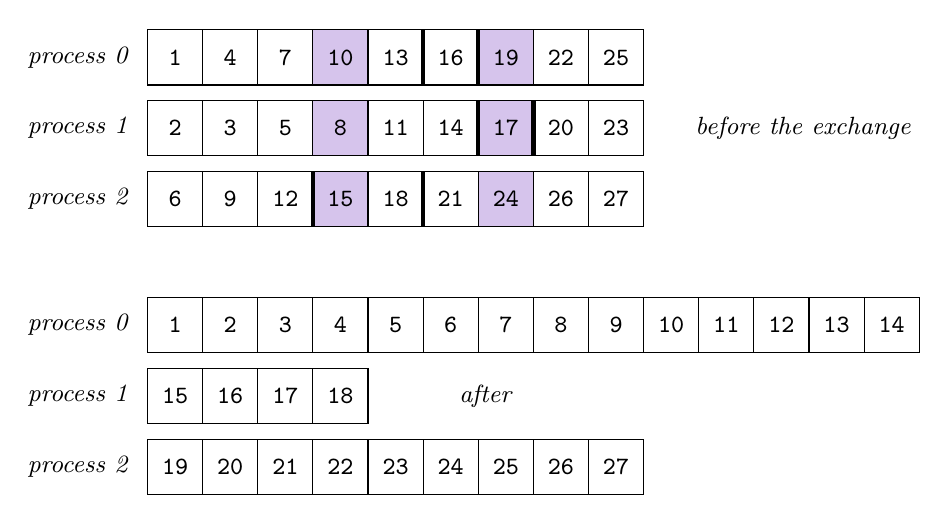
\begin{tikzpicture}[ads]
  \node[var,anchor=east] at (-6mm,-0mm) {process 0};
  \cells{a0}{0,-0mm}{1/cell,4/cell,7/cell,10/touched,13/cell,16/cell,19/touched,22/cell,25/cell}
  \node[var,anchor=east] at (-6mm,-9mm) {process 1};
  \cells{a1}{0,-9mm}{2/cell,3/cell,5/cell,8/touched,11/cell,14/cell,17/touched,20/cell,23/cell}
  \node[var,anchor=east] at (-6mm,-18mm) {process 2};
  \cells{a2}{0,-18mm}{6/cell,9/cell,12/cell,15/touched,18/cell,21/cell,24/touched,26/cell,27/cell}
  \draw[line width=1.6pt] (a0-4.north east) -- (a0-4.south east);
  \draw[line width=1.6pt] (a0-5.north east) -- (a0-5.south east);
  \draw[line width=1.6pt] (a1-5.north east) -- (a1-5.south east);
  \draw[line width=1.6pt] (a1-6.north east) -- (a1-6.south east);
  \draw[line width=1.6pt] (a2-2.north east) -- (a2-2.south east);
  \draw[line width=1.6pt] (a2-4.north east) -- (a2-4.south east);
  \node[var,anchor=west] at (66mm,-9mm) {before the exchange};
  \node[var,anchor=east] at (-6mm,-34mm) {process 0};
  \cells{b0}{0,-34mm}{1/cell,2/cell,3/cell,4/cell,5/cell,6/cell,7/cell,8/cell,9/cell,10/cell,11/cell,12/cell,13/cell,14/cell}
  \node[var,anchor=east] at (-6mm,-43mm) {process 1};
  \cells{b1}{0,-43mm}{15/cell,16/cell,17/cell,18/cell}
  \node[var,anchor=east] at (-6mm,-52mm) {process 2};
  \cells{b2}{0,-52mm}{19/cell,20/cell,21/cell,22/cell,23/cell,24/cell,25/cell,26/cell,27/cell}
  \node[var,anchor=west] at (36mm,-43mm) {after};
\end{tikzpicture}
\end{document}
